%!TEX root = ../Main.tex

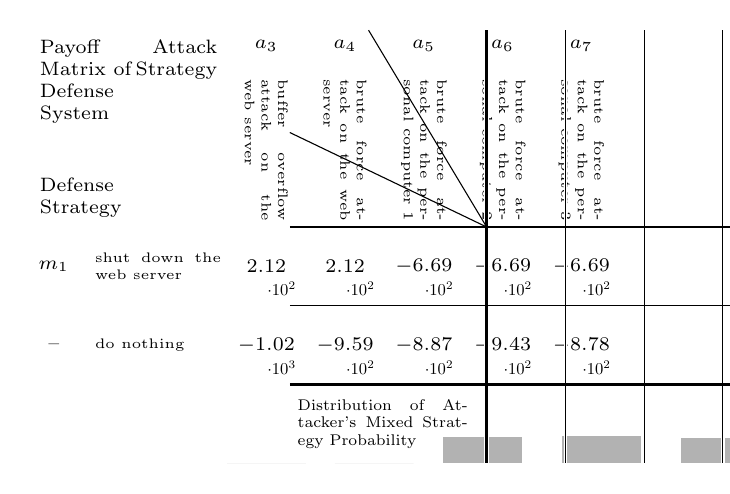
\begin{tikzpicture}
[line width = 0.4pt,
attack/.style = {anchor = north, align =center, font = \scriptsize},
attackdescription/.style = {anchor = west, align = left, font = \tiny, rotate = 270},
defense/.style = {align = center, font = \scriptsize},
defensedescription/.style = {anchor = west, align = left, font = \tiny}]
\linespread{1}
\node[anchor = north east, align = right, font = \scriptsize] at (2.5, 10) {Attack\\Strategy};
\node[anchor = south west, align = left, font = \scriptsize] at (0, 7.5) {Defense\\Strategy};
\node[anchor = north west, align = left, font = \scriptsize] at (0, 10) {Payoff\\Matrix of\\Defense\\System};
\node[defense] at (0.3, 7) {$m_{1}$};
\node[defensedescription] at (0.7, 7) {\parbox{1.6cm}{shut down the web server}};
\node[defense] at (0.3, 6) {--};
\node[defensedescription] at (0.7, 6) {\parbox{1.6cm}{do nothing}};
\node[attack] at (3, 10) {$a_{3}$};
\node[attackdescription] at (3, 9.5) {\parbox{1.8cm}{buffer overflow attack on the web server}};
\node[attack] at (4, 10) {$a_{4}$};
\node[attackdescription] at (4, 9.5) {\parbox{1.8cm}{brute force attack on the web server}};
\node[attack] at (5, 10) {$a_{5}$};
\node[attackdescription] at (5, 9.5) {\parbox{1.8cm}{brute force attack on the personal computer 1}};
\node[attack] at (6, 10) {$a_{6}$};
\node[attackdescription] at (6, 9.5) {\parbox{1.8cm}{brute force attack on the personal computer 2}};
\node[attack] at (7, 10) {$a_{7}$};
\node[attackdescription] at (7, 9.5) {\parbox{1.8cm}{brute force attack on the personal computer 3}};
\node[font = \scriptsize] at (3, 7) {$2.12$};
\node[anchor = south east] at (3.5, 6.5) {\scalebox{0.6}{$\cdot 10^{2}$}};
\node[font = \scriptsize] at (4, 7) {$2.12$};
\node[anchor = south east] at (4.5, 6.5) {\scalebox{0.6}{$\cdot 10^{2}$}};
\node[font = \scriptsize] at (5, 7) {$-6.69$};
\node[anchor = south east] at (5.5, 6.5) {\scalebox{0.6}{$\cdot 10^{2}$}};
\node[font = \scriptsize] at (6, 7) {$-6.69$};
\node[anchor = south east] at (6.5, 6.5) {\scalebox{0.6}{$\cdot 10^{2}$}};
\node[font = \scriptsize] at (7, 7) {$-6.69$};
\node[anchor = south east] at (7.5, 6.5) {\scalebox{0.6}{$\cdot 10^{2}$}};
\node[font = \scriptsize] at (3, 6) {$-1.02$};
\node[anchor = south east] at (3.5, 5.5) {\scalebox{0.6}{$\cdot 10^{3}$}};
\node[font = \scriptsize] at (4, 6) {$-9.59$};
\node[anchor = south east] at (4.5, 5.5) {\scalebox{0.6}{$\cdot 10^{2}$}};
\node[font = \scriptsize] at (5, 6) {$-8.87$};
\node[anchor = south east] at (5.5, 5.5) {\scalebox{0.6}{$\cdot 10^{2}$}};
\node[font = \scriptsize] at (6, 6) {$-9.43$};
\node[anchor = south east] at (6.5, 5.5) {\scalebox{0.6}{$\cdot 10^{2}$}};
\node[font = \scriptsize] at (7, 6) {$-8.78$};
\node[anchor = south east] at (7.5, 5.5) {\scalebox{0.6}{$\cdot 10^{2}$}};
\fill[black!30] (2.5, 4.5) -- (3.5, 4.5) -- (3.5, 4.5) -- (2.5, 4.5) -- cycle;
\shadowtext[font = \scriptsize] at (3, 5) {$0\%$};
\fill[black!30] (3.5, 4.5) -- (4.5, 4.5) -- (4.5, 4.5) -- (3.5, 4.5) -- cycle;
\shadowtext[font = \scriptsize] at (4, 5) {$0\%$};
\fill[black!30] (4.5, 4.5) -- (5.5, 4.5) -- (5.5, 4.8274) -- (4.5, 4.8274) -- cycle;
\shadowtext[font = \scriptsize] at (5, 5) {$33\%$};
\fill[black!30] (5.5, 4.5) -- (6.5, 4.5) -- (6.5, 4.8488) -- (5.5, 4.8488) -- cycle;
\shadowtext[font = \scriptsize] at (6, 5) {$35\%$};
\fill[black!30] (6.5, 4.5) -- (7.5, 4.5) -- (7.5, 4.8238) -- (6.5, 4.8238) -- cycle;
\shadowtext[font = \scriptsize] at (7, 5) {$32\%$};
\fill[black!30] (8.5, 7.5) -- (8.5, 6.5) -- (7.53, 6.5) -- (7.53, 7.5) -- cycle;
\shadowtext[font = \scriptsize] at (8, 7) {$100\%$};
\fill[black!30] (8.5, 6.5) -- (8.5, 5.5) -- (8.5, 5.5) -- (8.5, 6.5) -- cycle;
\shadowtext[font = \scriptsize] at (8, 6) {$0\%$};
\node[anchor = west] at (0, 5) {\scalebox{0.8}{\parbox{2.7cm}{\scriptsize Distribution of Attacker's Mixed Strategy Probability}}};
\node[anchor = west, rotate = -90] at (8, 10) {\scalebox{0.8}{\parbox{2.7cm}{\scriptsize Distribution of defense System's Mixed Strategy Probability}}};
\draw[line width = 1.2pt, white] (0, 6.5) -- (8.5 ,6.5);
\draw[line width = 1.2pt, white] (0, 5.5) -- (8.5 ,5.5);
\draw[line width = 1.8pt, white] (0, 5.5) -- (8.5 ,5.5);
\draw[line width = 1.8pt, white] (0, 7.5) -- (8.5 ,7.5);
\draw[line width = 1.2pt, white] (2.5, 10) -- (2.5, 4.5);
\draw[line width = 1.2pt, white] (3.5, 10) -- (3.5, 4.5);
\draw[line width = 1.2pt, white] (4.5, 10) -- (4.5, 4.5);
\draw[line width = 1.2pt, white] (5.5, 10) -- (5.5, 4.5);
\draw[line width = 1.2pt, white] (6.5, 10) -- (6.5, 4.5);
\draw[line width = 1.8pt, white] (7.5, 10) -- (7.5, 4.5);
\draw[line width = 1.8pt, white] (2.5, 10) -- (2.5,4.5);
\draw (0, 6.5) -- (8.5 ,6.5);
\draw (0, 5.5) -- (8.5 ,5.5);
\draw[line width = 1pt] (0, 5.5) -- (8.5 ,5.5);
\draw[line width = 1pt] (0, 7.5) -- (8.5 ,7.5);
\draw (2.5, 10) -- (2.5, 4.5);
\draw (3.5, 10) -- (3.5, 4.5);
\draw (4.5, 10) -- (4.5, 4.5);
\draw (5.5, 10) -- (5.5, 4.5);
\draw (6.5, 10) -- (6.5, 4.5);
\draw[line width = 1pt] (7.5, 10) -- (7.5, 4.5);
\draw[line width = 1pt] (2.5, 10) -- (2.5,4.5);

\draw (0, 8.7) -- (2.5, 7.5);
\draw (1, 10) -- (2.5, 7.5);
\end{tikzpicture}